\newpage
\section{\textbf{UNIT TEST CHO CÁC CHỨC NĂNG ĐÃ PHÂN TÍCH}}

\subsection{Unit test -- Chức năng quản lý mã khuyến mãi}

\textbf{Công cụ và phạm vi.}
Nhóm sử dụng \textbf{Jest} để viết và chạy unit test trong backend. Phạm vi trình bày của chương được giới hạn đúng theo hàm \texttt{validateCoupon(code, subtotal, userId)} đã phân tích ở Chương 4.

\textbf{Kết quả chạy unit test.}
Lệnh chạy test được sử dụng:
\begin{center}
	\texttt{npx jest tests/validateCoupon.test.js --verbose}
\end{center}
Kết quả chính thu được gồm:
\begin{itemize}
	\item \textbf{1 test suite passed}
	\item \textbf{9 tests passed}
	\item Khớp với các nhánh và điều kiện đã phân tích ở Chương 4 như mã rỗng, mã không tồn tại, coupon vô hiệu hóa, chưa hiệu lực, hết hạn, hết lượt dùng, vượt \texttt{perUserLimit}, chưa đạt \texttt{minimumOrderAmount} và trường hợp hợp lệ
\end{itemize}

\begin{figure}[H]
	\centering
	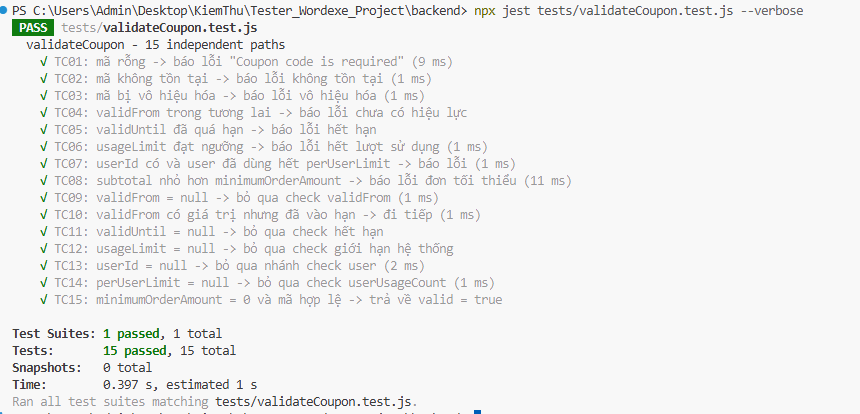
\includegraphics[width=\textwidth]{image/anhrchuongtestunittest/validate.png}
	\caption{Kết quả chạy unit test cho chức năng quản lý mã khuyến mãi}
	\label{fig:coupon-unit-test-result}
\end{figure}

\subsection{Unit test -- Chức năng đăng nhập}

\textbf{Công cụ và phạm vi.}
Nhóm sử dụng \textbf{Jest} để viết unit test cho hàm \texttt{login(\{ email, password \})} trong \texttt{authService}. Các phụ thuộc được mock trong bộ test gồm \texttt{userRepository.findByEmail}, \texttt{bcrypt.compare} và \texttt{jsonwebtoken.sign} để chỉ kiểm tra đúng luồng xử lý của hàm.

\textbf{Kết quả chạy unit test.}
Lệnh chạy test được sử dụng:
\begin{center}
	\texttt{npx jest tests/authService.login.test.js --verbose}
\end{center}
Kết quả chính thu được gồm:
\begin{itemize}
	\item \textbf{1 test suite passed}
	\item \textbf{3 tests passed}
	\item Khớp với ba nhánh đã phân tích ở Chương 4: email không tồn tại, email tồn tại nhưng mật khẩu sai, và đăng nhập thành công trả về \texttt{user} cùng \texttt{token}
\end{itemize}

\begin{figure}[H]
	\centering
	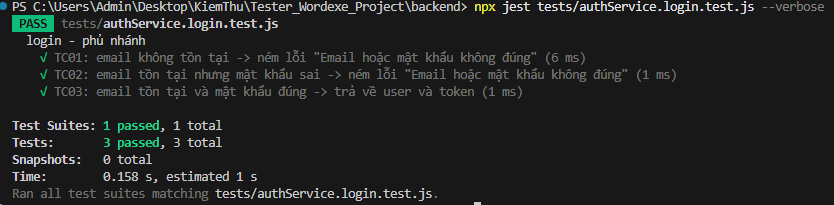
\includegraphics[width=\textwidth]{image/anhrchuongtestunittest/dangnhap.png}
	\caption{Kết quả chạy unit test cho chức năng đăng nhập}
	\label{fig:login-unit-test-result}
\end{figure}
